\title{Machine Learning Spring 2019 HW3}
\author{
        Yueh Cheng Liu \\
        National Taiwain University\\
}
\date{\today}
\documentclass[12pt]{article}
\usepackage{amsmath,amssymb}
\usepackage{bbm}
\usepackage{graphicx}
\usepackage{mathtools}
\usepackage{bm}
\DeclareMathOperator{\E}{\mathbb{E}}
\begin{document}
\maketitle

% \begin{abstract}
% This is the paper's abstraasdsadsct \ldots
% \end{abstract}

\section*{1}
Minimize $\sum_{k=1}^K \mu_k^2$
\begin{equation*}
\begin{split}
    (\sum_{k=1}^K \mu_k^2)(\sum_{k=1}^K 1^2) &= K \sum_{k=1}^K \mu_k^2 \\
    &\geq (\sum_{k=1}^K 1\mu_k)^2 \\
    &= 1
\end{split}
\end{equation*}
By Cauchy–Schwarz inequality, $\sum_{k=1}^K \mu_k^2 = \frac{1}{K}$ when 
$\frac{\mu_1}{1} = \frac{\mu_2}{1} = ... = \frac{\mu_K}{1} = \frac{1}{K} \geq 0$.
The maximum $1 - \sum_{k=1}^K \mu_k^2 = \frac{K-1}{K}$.

\section*{2}
Let $a=\mu_+$ and $b=\mu_-$, $a=1-b$.
The gini index is
\begin{equation*}
\begin{split}
    1 - a^2 - b^2 &= 1 - a^2 - (1-a)^2 \\
    &= 1 - a^2 - 1 + 2a - a^2 = 2a - 2a^2
\end{split}
\end{equation*}
And the squared regression error is 
\begin{equation*}
\begin{split}
    a(1-(a - (1-a)))^2 + (1-a)(-1 - (a-(1-a)))^2 
    &= a(2-2a)^2 + (1-a)(2a)^2 \\
    &= 4a(1-2a+a^2) + 4a^2(1-a) \\
    &= 4[a-2a^2 + a^4 + a^2 - a^3] = 4a - 4a^2
\end{split}
\end{equation*}
which is the $2 \cdot$ gini-index.

\section*{3}
The probabilty of a example not been choosen at all is 
\begin{equation*}
\begin{split}
    (1 - \frac{1}{N})^{N'} &= \frac{1}{(1+\frac{1}{N-1})^{Np}} \\
    &\simeq e^{-p}
\end{split}
\end{equation*}
So the total number of example not been choosen is $Ne^{-p}$.

\section*{4}
If one example is wrong by $G$, then at least $\frac{K+1}{2}$ $g$ is wrong. Thus, to make the largest $E_{out}$, seperate $\sum_{k=1}^K e_k$ to the first $\frac{K+1}{2}$ $g$
which result of $E_{out} \leq \frac{2}{K+1} \sum_{k=1}^K e_k$.

\section*{5}
\begin{equation*}
\begin{split}
    \alpha_t &= \frac{\sum_{n=1}^N g_t(x_n)(y_n - s_n)}{\sum_{n=1}^N g_t^2(x_n)} \\
    &= \frac{\sum_{n=1}^N 11.26y_n}{11.26^2 N} \\
    &= \frac{\sum_{n=1}^N y_n}{11.26N}
\end{split}
\end{equation*}
\section*{6}
\begin{equation*}
\begin{split}
    \sum_{n=1}^{N} s_n g_t(x_n) &= \sum_{n=1}^{N} (s_n + \alpha_t g_t(x_n)) g_t(x_n) \\
    &= \sum_{n=1}^{N} s_n  g_t(x_n) + \alpha_t g_t^2(x_n) \\
    &= \sum_{n=1}^{N} s_n  g_t(x_n) + \alpha_t \sum_{n=1}^{N} g_t^2(x_n) \\
    &= \sum_{n=1}^{N} s_n  g_t(x_n) + \frac{\sum_{n=1}^N g_t(x_n)(y_n - s_n)}{\sum_{n=1}^N g_t^2(x_n)} \sum_{n=1}^{N} g_t^2(x_n) \\
    &= \sum_{n=1}^{N} s_n  g_t(x_n) + \sum_{n=1}^N g_t(x_n)(y_n - s_n) \\
    &= \sum_{n=1}^N g_t(x_n)y_n
\end{split}
\end{equation*}

\section*{7}
Assume that a polynomial $g_1$ is a minimizer of $\sum_{n=1}^{N}(y_n -s_n - g_1(x_n))^2 = \sum_{n=1}^{N}(y_n - g_1(x_n))^2$.
$\alpha_1$ is the minimizer of $\sum_{n=1}^{N}(y_n - \alpha_1g_1(x_n))^2$ but not equals to $1$.  \\
Since $g_1(x_n)$ is polynomial and so does $g'_1(x_n)$ where $g'_1 = \alpha_1g_1 \neq g_1$ , 
$\sum_{n=1}^{N}(y_n - g'_1(x_n))^2 < \sum_{n=1}^{N}(y_n - g_1(x_n))^2$ is a contradiction of $g_1$ being the minimizer of $\sum_{n=1}^{N}(y_n - g_1(x_n))^2$.


\section*{8}
$w_0 = d-1$ and $w_i = +1$ for $i=1...d$. \\
If at least one of $x_i$ is $+1$ and others are $-1$, the result $\sum w_i x_i \geq d-1 + 1 - (d-1) = 1$.
And if all $x_i = -1$, the result $\sum w_i x_i = (d-1) - d = -1$.

\section*{9}
The gradient of weights in last layer 
\[
    \frac{\partial e_n}{\partial w_{i,1}^L}
    = -2 (y_n - tanh(s_1^L)) tanh'(s_1^L) x_i^{(L-1)}
\]
is $0$ because $x_i^{(L-1)}=0$.
Also the gradient of weights in first layer
\[
    \frac{\partial e_n}{\partial w_{i,j}^l}
    = \sum_k x_i (\delta_k^{l+1}) (w_{j,k}) (tanh'(s_j^l))
\]
is $0$ because the gradient of next layer $\delta_k^{l+1}=0$.

\section*{10}
\begin{equation*}
\begin{split}
\frac{\partial e}{\partial s_k^{(L)}} &= \frac{\partial -\sum_{i=1}^{K} v_i \ln q_i}{\partial s_k^{(L)}} \\
&= - \frac{\partial v_k \ln q_k + \sum_{i=1, i\neq k}^{K} v_i \ln q_i}{\partial s_k^{(L)}} \\
&= - \frac{\partial v_k(\ln e^{s_k^L} - \ln\sum_{j=1}^K e^{s_j^L}) - \sum_{i=1, i\neq k}^{K} v_i(\ln e^{s_i^L} - \ln\sum_{j=1}^K e^{s_j^L})}{\partial s_k^{(L)}} \\
&= - v_k + v_k \frac{e^{s_k^L}}{\sum_{j=1}^K e^{s_j^L}} + - \sum_{i=1, i\neq k}^{K} v_i \frac{e^{s_k^L}}{\sum_{j=1}^K e^{s_j^L}} \\
&= -v_k + q_k
\end{split}
\end{equation*}

\section*{11}
\begin{center}
    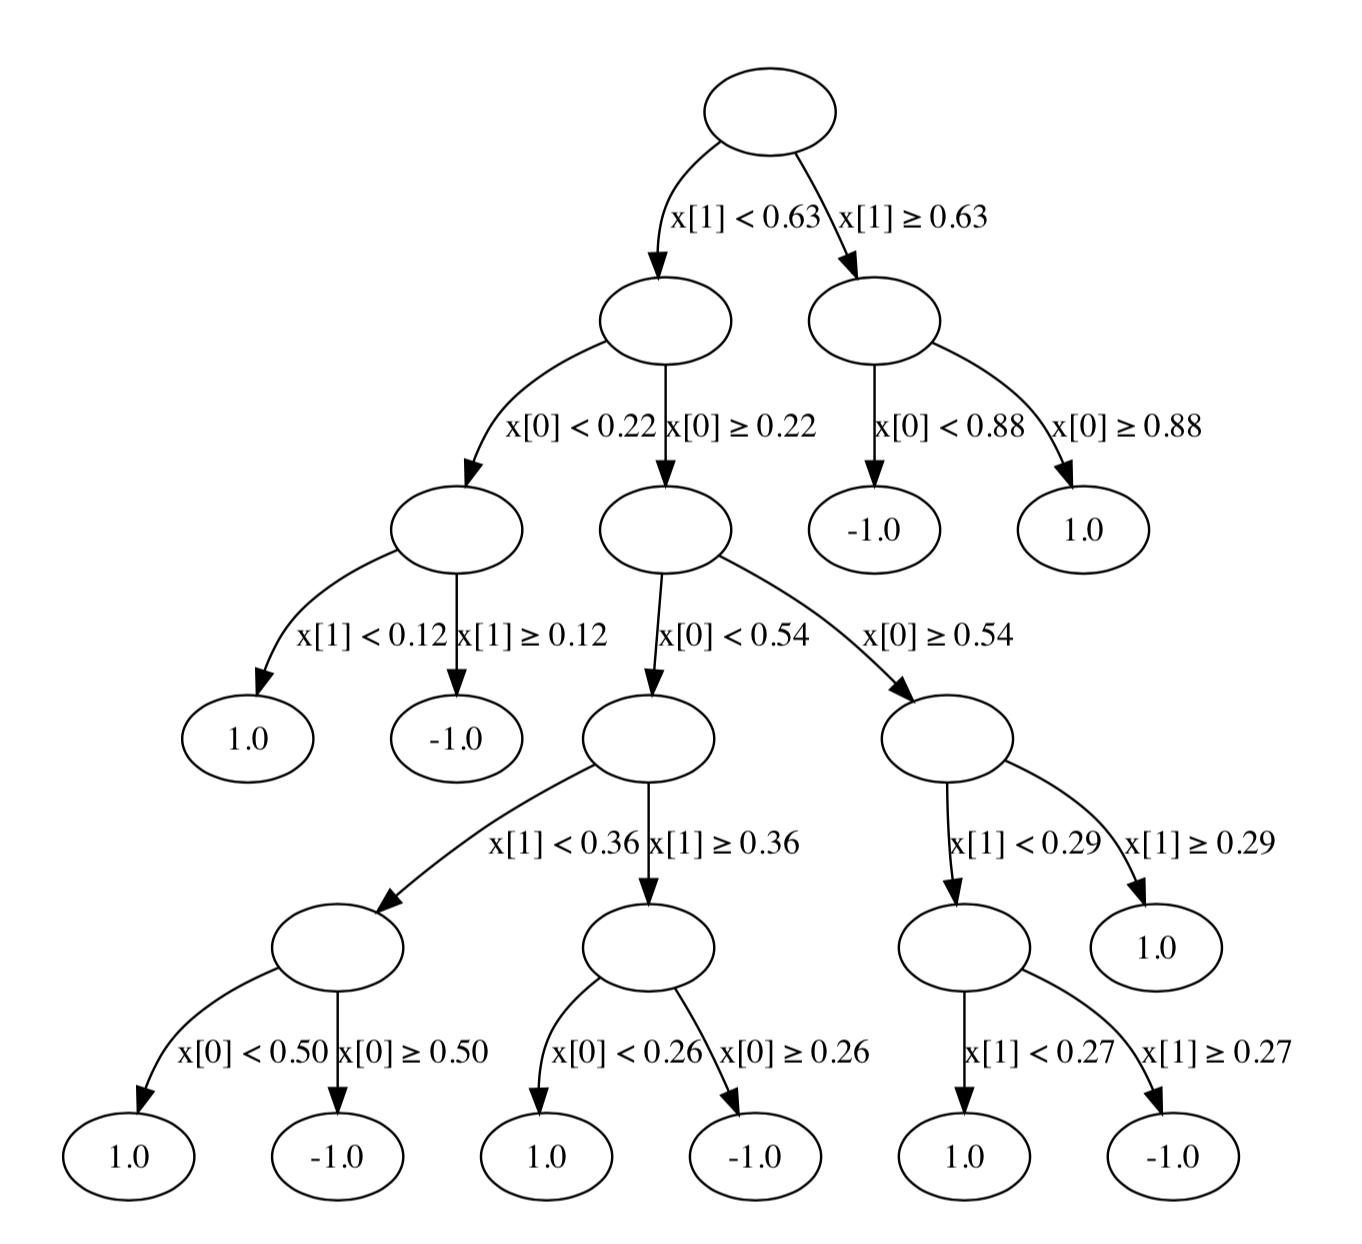
\includegraphics[scale=0.4]{p11.png}
\end{center}

\section*{12}
$E_{in} = 0.0$ \\
$E_{out}  = 0.126$

\section*{13}
\begin{center}
    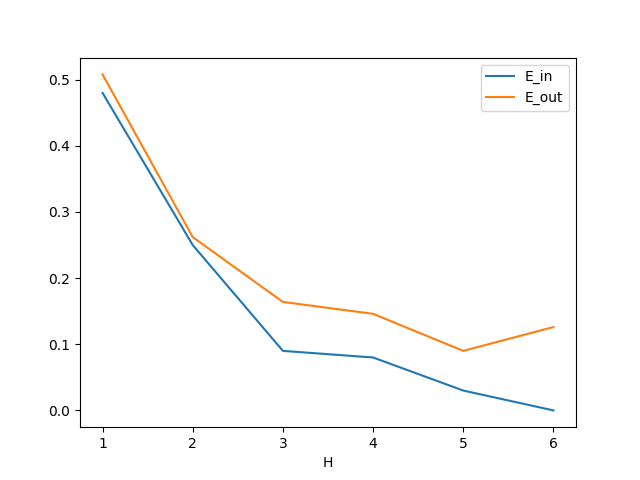
\includegraphics[scale=0.5]{p13.png}
\end{center}

\begin{itemize}
\item Both $E_{in}$ and $E_{out}$ decrease with larger $H$. 
\item When $H=1$ (directly output the $y_n$ appears the most in training data), 
both $E_{in}$ and $E_{out}$ is around $0.5$. This means that training and testing data are balance.
\item With full grown tree $H=6$, $E_{in}$ becomes $0$, which is the property of decision tree.
\item $E_{out}$ with $H=5$ is lower than $H=6$. This may be caused by overfitting.
\end{itemize}

\section*{14}
\begin{center}
    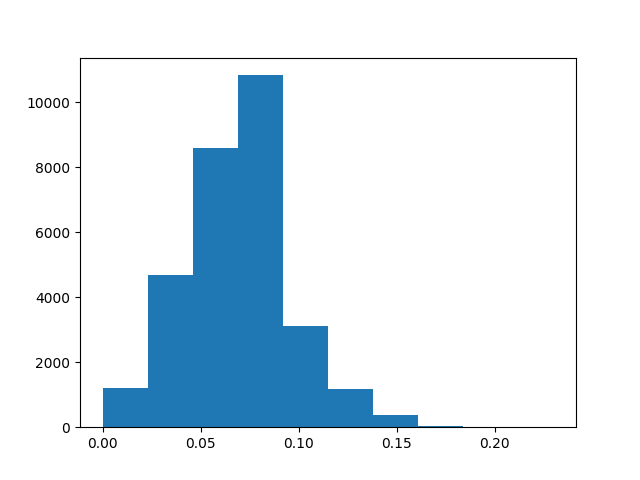
\includegraphics[scale=0.5]{p14.png}
\end{center}

\section*{15}
\begin{center}
    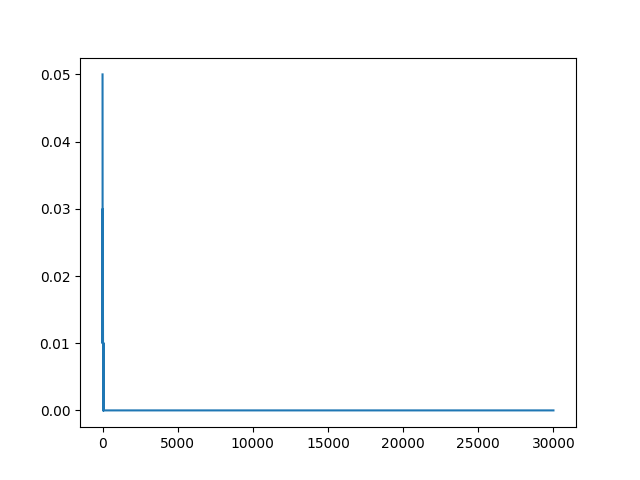
\includegraphics[scale=0.5]{p15.png}
\end{center}

\section*{16}
\begin{center}
    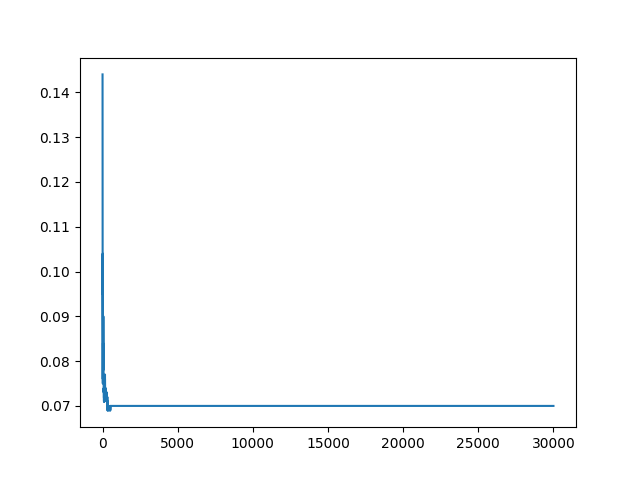
\includegraphics[scale=0.5]{p16.png}
\end{center}
\begin{itemize}
\item Both error converge early compares to $T=30000$. 
\item The error rate unlike $E_{in}$ is $0$ but converge at $0.07$
\item The error rate has slightly increase after $t=500$.
\end{itemize}

\section*{17}
\section*{18}
\end{document}


